
\section{Introduction}

Nowadays, location-based networks, e.g., Foursquare and Yelp, are becoming more and more popular. 
These platforms provide kinds of point of interests (POIs) such as hotels, restaurants, and markets, which makes our lives much easier than before. 
Meanwhile, the problem of ``where to go'' starts to bother people, since it is time-consuming for people to find their desired places from so many POIs. 
POI recommendation appears to address such a problem by helping users filter out uninteresting POIs and saving their decision-making time \cite{ye2011exploiting,gao2015content}.

Among the existing research from POI recommendation communities, Matrix Factorization (MF) techniques draws a lot of attention \cite{cheng2011exploring,cheng2012fused,yang2013sentiment}, and it has proven to be attractive in many recommendation applications \cite{koren2009matrix,chen2014context,koenigstein2011yahoo,chen2016capturing}. 
However, existing MF approaches train the recommendation model in a centralized way. 
That is, the recommender system, actually the organization who built it, first needs to collect the action data of all the users on all the POIs, and then trains a MF model. 
The shortcomings of this kind of centralized MF methods are mainly three-folds.
(1) \textit{High cost of resources}. 
Centralized MF not only needs large storage to store the collected user action data on POIs, but also requires huge computing resources to train the model, especially when datasets are large. 
(2) \textit{Low model training efficiency}. Centralized MF model is trained on a single machine or a cluster of machines. 
Thus, the model training efficiency is restricted to the number of machines available. 
(3) \textit{Shallow user privacy protection}. 
In recommender systems, user privacy is an importance concern \cite{canny2002collaborative}, especially in POI scenarios. 
Most people do not want to release their activities on location based network, not only to other people, but also to the platforms, for privacy concerns. 
However, centralized MF trains model on the basis of having all the users' activities data. 
In fact, the safest way is that users' data are kept in their own hand, without sending them to anyone or any organization (platform). 

 
\begin{figure}[!tp]
\centering
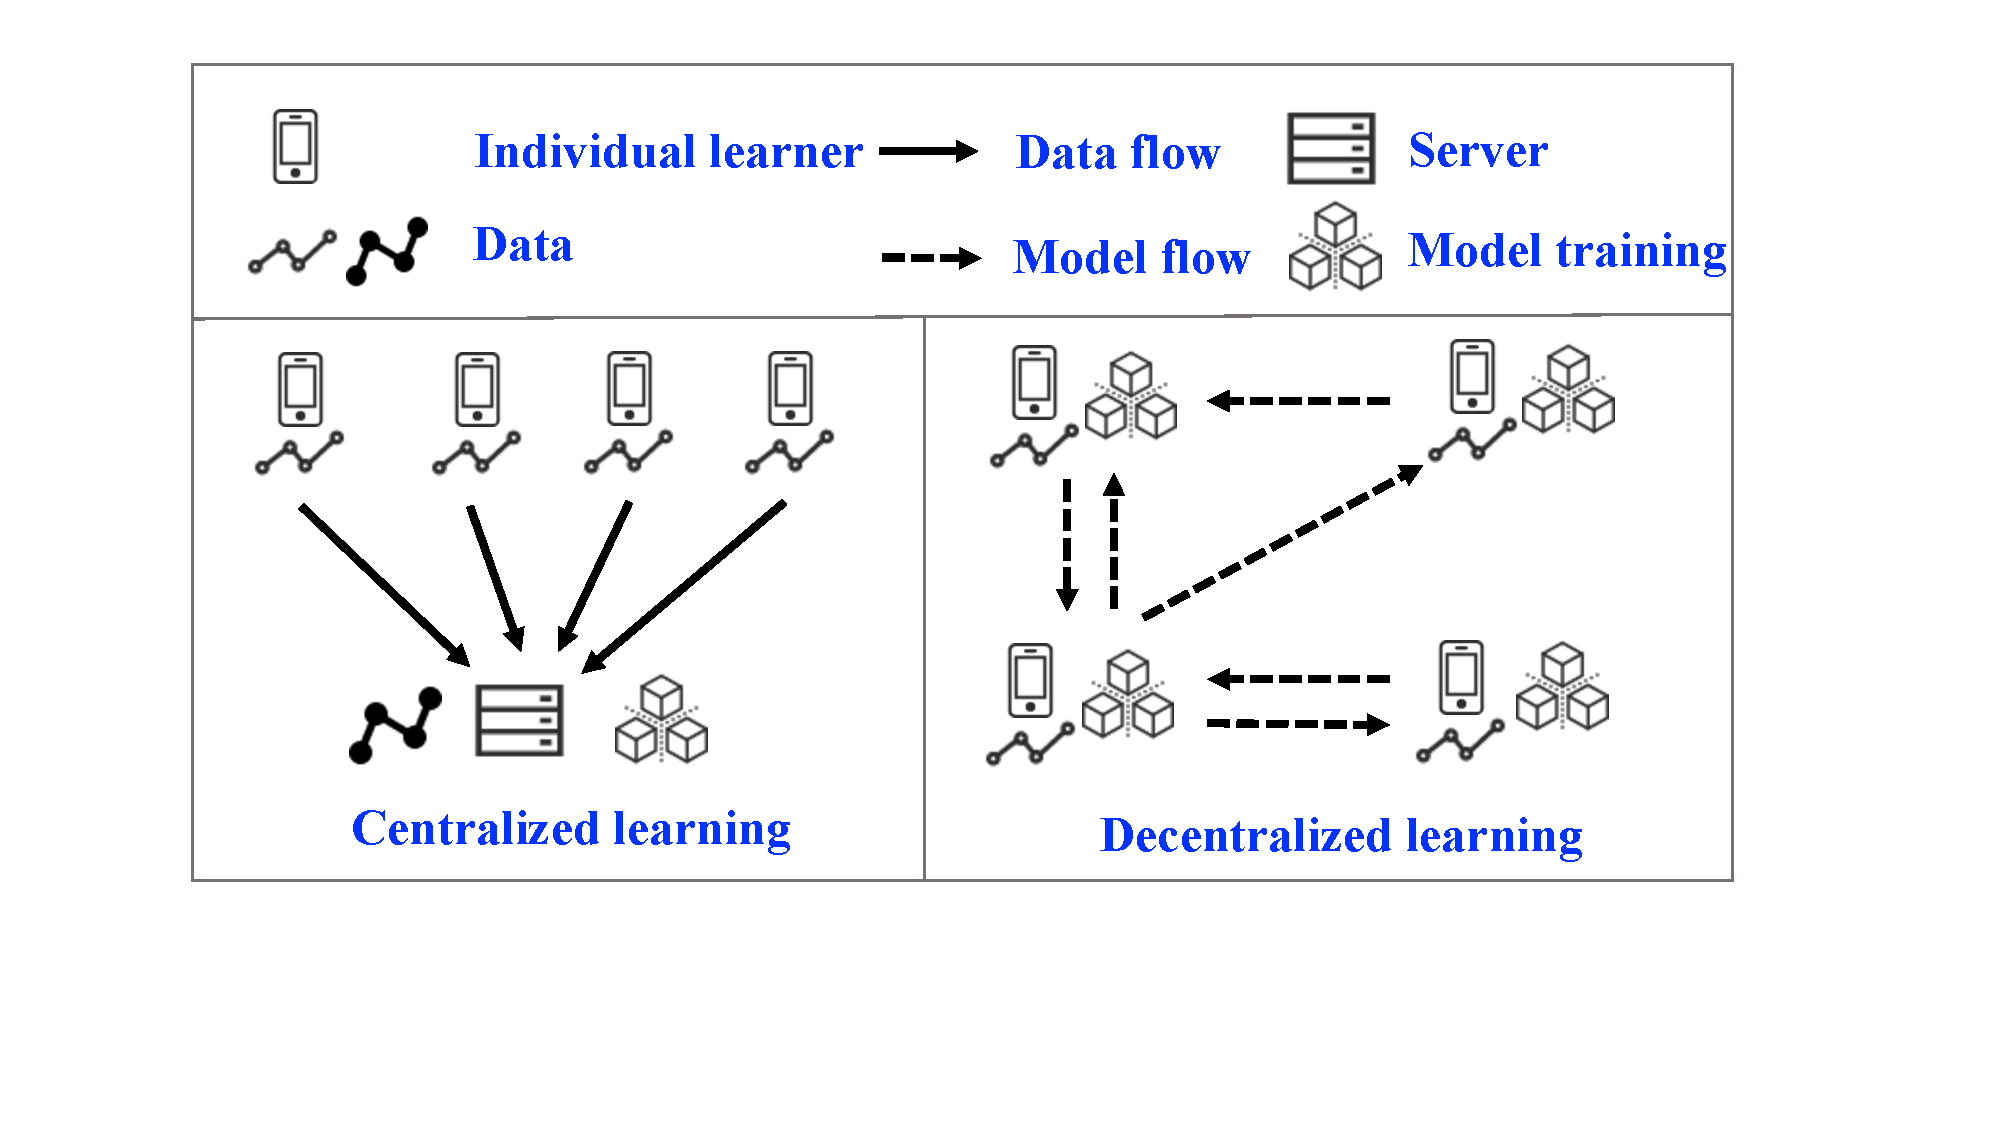
\includegraphics[width=7cm]{figures/decentralize}
\vskip -0.1in
\caption{Comparison between centralized learning and decentralized learning.}
\label{framework}
\vskip -0.15in
\end{figure}
 
To solve the above problems caused by centralized training of MF, we propose Decentralized MF (DMF) framework. 
That is, instead of training user and item latent factors in a centralized way by obtaining all the ratings, we train MF model in each user's end, e.g., user's cell phone and Pad.  
Figure \ref{framework} shows the difference between centralized and decentralized learning. 
DMF treats each user's device as an autonomous learner (individual computation unit). 
As we know, the essence of MF is that user and item latent factors are learnt collaboratively, so should be DMF. 
Three key challenges exist when making users collaborate in DMF meanwhile preserving user privacy. 
The first challenge is \textit{which user should be communicated}. 
We answer this question by analyzing the data in POI recommendation scenarios, and propose nearby user communication on user adjacent graph, which is built based on users' geographical information. 
Along with this, the second challenge naturally appears: \textit{how far should users communicate with their neighbors}. 
To address this, we present a random walk method to enhance local user communication. 
That is, we use random walk technique to intelligently select users' high-order neighbors instead of only their direct neighbors. 
The third and also the most serious challenge is \textit{what information should users communicate with each other} without leaking their data privacy. 
To solve this challenge, we decompose item preference into global (common) and local (personal) latent factors, and allow users communicate with each other by sending the gradients of the global item latent factors. 

Our proposed DMF framework successfully deals with the shortcomings of centralized MF.  
(1) Each user only needs to store his own latent factor, and items' latent factors. 
%For example, it only needs 61MB memories for each user to save all the parameters to train a DMF model, with 1 million items and 16 latent dimensions. 
The computation is also cheap: each user only need to update the corresponding user and item latent factors when he (his neighbors) rates (rate) an item. 
(2) Since each user updates the DMF model on his own side, it can be taken as a distributed learning system with \#users as \#machines, which makes the model efficient to train. 
(3) The ratings of each user on items are still kept on one's own hand, which avoids user's privacy being disclosed. 


We summarize our main contributions as follows: 
\begin{itemize}
\item We propose a novel DMF framework for POI recommendation, which is scalable and is able to preserve user privacy. 
To our best knowledge, it is the first attempt in literature. 
\item We propose an efficient way to train DMF. Specifically, when a user rates an item on his side, the user and item gradients are first calculated. We then present a random walk based technique for users to send the item gradient to their neighbors. Finally, the correspoding user/item latent factors are updated using stochastic gradient descent. 
\item Experimental results conducted on two real-world datasets demonstrate that DMF can achieve even better performance compared with the classic and state-of-the-art latent factor models in terms of precision and recall. 
Parameter analysis also shows the effectiveness of our proposed random walk based optimization method. 
\end{itemize}

